\documentclass{article}
\usepackage[utf8]{inputenc}
\usepackage[italian]{babel}
\usepackage{graphicx}

\title{Determinazione della caratteristica IV di due
resistenze di valore normale diverso, di una
lampadina ad incandescenza e di un diodo e
applicazione del metodo voltamperometrico per la
misura della resistenza}
\author{O. D. Caputo, C. Crismale, E. Panteghini}
\date{~}

\begin{document}

\maketitle

\section{Introduzione}
L’esperienza si basa sul confronto di due diversi processi di misura di una resistenza
incognita, cioè il metodo del voltmetro “a valle” ed “a monte” dell’amperometro. In modo da ridurre il più possibile la correlazione tra le misure effettuate, entrambi i metodi utilizzano due strumenti
di misura diversi, possibilmente anche di due aziende differenti, al fine da semplificare l’analisi statistica dei dati). Dalla presenza di voltmetro ed amperometro all'interno di questi due configurazioni di misura, i due metodi vengono genericamente
denominati come “voltamperometrici”.
Va premesso che la definizione di resistenza usata è quella di dispositivo
elettrico per cui la relazione caratteristica, che lega intensità di corrente che
scorre nel dispositivo e la tensione ai suoi capi, è proprio la legge di Ohm:

\begin{equation}
    V = IR
\end{equation}

Tale premessa, la cui validità è anche obiettivo dell’esperienza, non è scontata
come si potrà evincere dalla relazione caratteristica diversa di lampadina a incandescenza
e diodo (vedi Appendice) La necessità di due metodi diversi nasce
dal fatto che è impossibile inserire contemporaneamente il voltmetro in parallelo
con la resistenza incognita e l’amperometro in serie con la stessa. Il metodo “a valle” prevede, infatti, il voltmetro in parallelo con la resistenza e il loro parallelo
in serie con l’amperometro. Invece, il metodo “a monte” prevede il voltmetro
in parallelo con la serie composta da resistenza incognita e voltmetro. Risulta
rilevante specificare che nel primo caso solo la tensione letta dal voltmetro
coincide con quella realmente ai capi della resistenza (mentre la corrente che
scorre nell’amperometro, e quindi letta, sarà influenzata dalla presenza del voltmetro all'interno del circuito). Analogamente, nel metodo a valle solo la corrente letta è quella che
realmente scorre nella resistenza; la tensione misurata dal voltmetro è quella
ai capi della serie, quindi diversa dal valore reale di quella ai capi della sola
resistenza. Ne consegue che il rapporto tra la tensione e l’intensità di corrente
misurata dagli strumenti, in entrambi i casi, non coincide con il valor vero della
resistenza. Tuttavia, attraverso le leggi di Kirchhoff è possibile risalire all’esatta
espressione della resistenza incognita, risolvendo il circuito. Ricaviamo quindi
che per il circuito con voltmetro a valle dell’amperometro:
\begin{equation}
    R = \frac{V_V}{I_R}= \frac{V_V}{I_A}(1+\frac{R}{R_V})> \frac{V_V}{I_A} = R_{Mis}
\end{equation}
Da cui si evince che il valore misurato dagli strumenti è sempre più piccolo del
valor vero. Al contrario, per il metodo del voltmetro a monte dell’amperometro:
\begin{equation}
    R = \frac{V_V}{I_R}-R_A <\frac{V_V}{I_R} = R_{Mis}
\end{equation}
In questo caso, si ha che la resistenza misurata è sistematicamente maggiore del
valore vero. Sempre usando le leggi di Kirchhoff si ricavano le relazioni tra il valor
vero e quello misurato nei due casi, riportati qui sotto. Va specificato che nei
casi limite in cui la resistenza del voltmetro è molto maggiore di quella incognita
e quello in cui la resistenza dell’amperometro sia trascurabile (rispettivamente
per il metodo a valle e a monte), il valore misurato non è apprezzabilmente
differente dal valor vero.
\begin{equation}
    R = \frac{1}{\frac{I_A}{V_V}-\frac{1}{R_V}}
\end{equation}
\begin{equation}
    R = \frac{V_V}{I_A}-R_A
\end{equation}
Il calcolo delle incertezze relative sulla resistenza in ciascun metodo fornisce un
discriminante su quale dei due usare. Per il metodo a valle:
\begin{equation}
    \varepsilon_R = \frac{\Delta R}{R} = \frac{R}{R + R_V}
\end{equation}
mentre a monte:
\begin{equation}
    \varepsilon_R = \frac{|\Delta R|}{R} = \frac{R_A}{R}
\end{equation}
Uguagliando al limite le due incertezze relative si ottiene il valore al di sopra
del quale conviene usare il metodo a monte e, viceversa, al di sotto il metodo a
valle, ossia $R = \sqrt{R_A R_V}$

\section{Illustrazione del metodo di misura e della strumentazione}
\subsection{Strumentazione dell'esperimento}
L'apparato sperimentale adoperato per l'esperienza consiste in:
\begin{itemize}
    \item[-] Generatore di tensione continua variabile tra 0 e 20 V
    \item[-] Tester analogico (in funzione di amperometro)
    \item[-] Tester digitale (in funzione di voltmetro)
\end{itemize}
I dispositivi circuitali utilizzati per la composizione dei circuiti si dividono
in:
\begin{itemize}
    \item[-] n.1 resistore (100$\Omega$)
    \item[-] n.1 resistore (2.2 M$\Omega$)
    \item[-] n.1 diodo ad emissione luminosa (LED)
    \item[-] n.1 lampadina
\end{itemize}
I circuiti sono stati assemblati mediante breadboard e fili conduttori.

\subsection{Metodo di misura}
L’esperienza consiste nel misurare le resistenze di resistori aventi diversa
intensità, applicando due differenti metodi voltamperometrici: a valle e a monte. Il metodo
voltamperometrico è utilizzato per misurare la resistenza di un resistore
considerando sia la corrente che attraversa il resistore, utilizzando la legge di
Ohm, che la d.d.p. ai suoi capi. Le misure si effettuano mediante voltmetro
e amperometro posizionati in modo da non avere contemporaneamente il voltmetro
in parallelo alla resistenza e l’amperometro in serie. E' stato realizzato il
circuito sulla breadboard impiegando le resistenze sopra citate. Successivamente,
si è collegato il circuito ad un generatore di f.e.m. e si è effettuata la raccolta
dati, seguendo i procedimenti di seguito descritti:
\subsubsection{Metodo del voltmetro a valle dell’amperometro}
Il circuito è composto da quattro componenti: generatore di f.e.m., resistore in
parallelo al voltmetro e amperometro a valle del voltmetro cioè: il voltmetro
misurerà la tensione ai capi della resistenza incognita e l’amperometro che si
trova a monte misurerà la corrente che scorre attraverso sé stesso che risulterà
differente da quella che scorre nella resistenza incognita. In particolare, per
effettuare le misure delle correnti passanti attraverso la lampadina e il diodo
LED è stato applicato unicamente il metodo a valle.
\subsubsection{Metodo del voltmetro a monte dell’amperometro}
Il circuito è composto da quattro componenti: generatore di f.e.m., resistore e
amperometro in serie, in parallelo al voltmetro. In questo modo, il voltmetro
sarà a monte dell’amperometro: il voltmetro misurerà la tensione ai capi della serie resistenza incognita e amperometro, mentre l’amperometro misurerà la
corrente che circola nella resistenza incognita.
\section{Procedure di misura ed analisi dei dati}
Per l’esecuzione della misura si à adoperato il generatore f.e.m. ruotando l’indicatore
in modo da leggere sul voltmetro la tensione desiderata. Si è scelto
di far variare la tensione fino al valore di 20 V. Fissato il valore della tensione,
si è utilizzato il tester analogico: immettendo gli spinotti negli ingressi prestabiliti
per ottenere il valore del fondo scala inizialmente di 50 mA. Effettuata
la misura sono stati tabulati i valori segnati dallo strumento su foglio \emph{Excel}.
Nel momento in cui l’indicatore dell’amperometro raggiunge il valore del fondo
scala, è necessario variare quest’ultimo, passando al successivo: 500 mA. L’interpretazione
del valore indicato dall’amperometro sulla scala graduata varia a
seconda del fondo scala considerato: in particolare, il multimetro ha una scala
graduata divisa in 5 parti ciascuna avente 10 tacche. Il valore massimo indicato
coincide con quello del fondo scala
La modalità di raccolta dati ed esecuzione dell’esperienza è stata ripetuta per
il metodo a monte sia per la costruzione del circuito che per le effettive procedure
di misura, come, per esempio, la necessità di adoperare fondo scala diversi in
corrispondenza di valori limite. Differentemente, però, rispetto al metodo a
valle l’amperometro `e inserito nel circuito in posizioni distinte. L’esperienza è stata ripetuta poi per il resistore da 2.2 M$\Omega$ con uguali modalità, unicamente è stato sufficiente adottare una corrente di fondo scala pari a 50 $\mu$A.
Nelle seguenti figure sono elencati i dati e relative incertezze:
\begin{figure}
    \begin{center}
        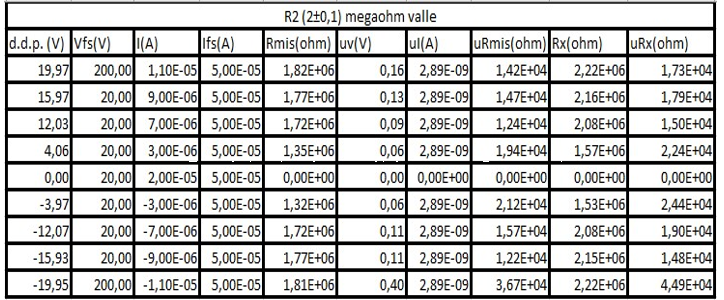
\includegraphics[width=\linewidth]{rel1-tabella_r2valle.png}
    \end{center}
    \caption{Dati relativi alla misura della resistenza di valore nominale di 2.2M$\Omega$:
tensione ai capi, tensione di fondo-scala dello strumento, corrente, corrente di
fondo-scala dello strumento, rapporto tra tensione e corrente misurate ($R_{MIs}$),
resistenza e relative incertezze, con metodo a valle}
    \label{figura1}
\end{figure}
Passando al calcolo delle incertezze, va premesso che quelle relative al processo
di misura della tensione da parte del voltmetro e dell’intensità di corrente da parte dell’amperometro sono determinate considerando la natura (analogica o digitale) dello strumento e le specifiche fornite dal costruttore:

\begin{figure}
    \centering
    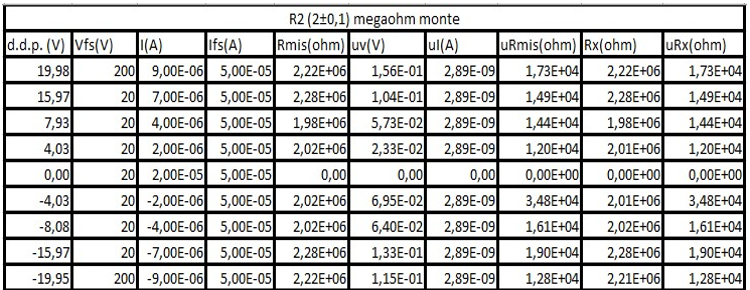
\includegraphics[width=\linewidth]{rel1-tabella_r2monte.png}
    \caption{Dati relativi alla misura della resistenza di valore nominale di 2.2M$\Omega$:
tensione ai capi, tensione di fondo-scala dello strumento, corrente, corrente di
fondo-scala dello strumento, rapporto tra tensione e corrente misurate ($R_{mis}$),
resistenza e relative incertezze, con metodo a monte}
    \label{figura2}
\end{figure}
\begin{equation}
    u_{I_A} = \frac{1}{\sqrt{3}}\frac{CP I_{FS}}{100}
\end{equation}
con CP classe di precisione dello strumento dell’1$\%$ e
\begin{equation}
    u_{V_V} = \frac{1}{\sqrt{3}}(\%lettura + 1digit)
\end{equation}
Considerando così note le incertezze su tensione e intensità di corrente, si possono ricavare quelle sulle altre grandezze usando la formula di propagazione degli errori. Risulta quindi che:
\begin{equation}
    u_R^2 = \Bigl (\frac{R_V}{R_V-R_{Mis}}\Bigl )^4 u_{R_{Mis}} + \Bigl (\frac{R_{Mis}}{R_V-R_{Mis}}\Bigl )^4 u_{R_V}^2
\end{equation}
per il metodo a valle;
\begin{equation}
    u_R^2 = u_{R_{Mis}}^2 + u_{R_A}^2
\end{equation}
per il metodo a monte, avendo considerato nelle equazioni precedenti che:
\begin{equation}
    u_{R_{Mis}} = \Bigl (\frac{1}{I_A} \Bigl )^2 u_{V_V}^2 + \Bigl (-\frac{V_V}{I_A^2} \Bigl )^2 u_{I_A}^2
\end{equation}
\section{Presentazione dei risultati e conclusioni}
Utilizzando il metodo voltamperometrico, si è misurato due volte il valore di due differenti resistenze, ognuno dei quali accompagnato dalla relativa incertezza sperimentale.
\begin{figure}
    \centering
    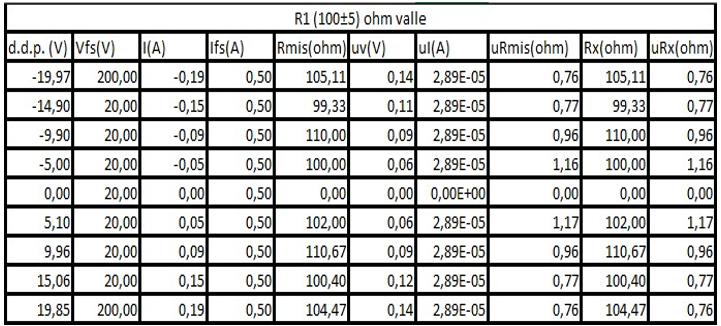
\includegraphics[width=\linewidth]{rel1-tabella_r1valle.png}
    \caption{Dati relativi alla misura della resistenza di valore nominale di 100$\Omega$:
tensione ai capi, tensione di fondo-scala dello strumento, corrente, corrente di
fondo-scala dello strumento, rapporto tra tensione e corrente misurate ($R_{Mis}$),
resistenza e relative incertezze, con metodo a valle}
    \label{figura3}
\end{figure}
La misura effettuata mediante il metodo voltamperometrico a
valle ha restituito un valore sperimentale della resistenza più piccola pari a
(101.77 ± 0.33) $\Omega$; d’altra parte il metodo a monte ha restituito (104.68 ± 0.76)
$\Omega$. Analogamente, la misura dell’altra resistenza ha restituito i valori di (2.24
± 0.03) M$\Omega$ con il metodo a monte e (1.77 ± 0.02) M$\Omega$ . Come è possibile constatare dalle incertezze sperimentali, i metodi più accurati per la misura di un resistore sono rispettivamente: quello a valle per resistenze di piccolo valore e quello a monte per resistenze più grandi. Per i risultati riguardanti la lampadina e il led si rimanda all’appendice seguente.
Qui si riportano i grafici che verificano la legge di Ohm per le due resistenze,
ognuno di loro fatto usando i dati ottenuti con entrambi i metodi, come indicato.
\begin{figure}
    \centering
    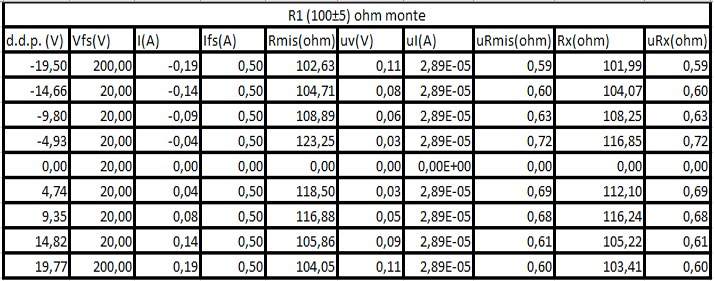
\includegraphics[width=\linewidth]{rel1-tabella_r1monte.png}
    \caption{Figura 4: Dati relativi alla misura della resistenza di valore nominale di 100$\Omega$:
tensione ai capi, tensione di fondo-scala dello strumento, corrente, corrente di
fondo-scala dello strumento, rapporto tra tensione e corrente misurate ($R_{Mis}$),
resistenza e relative incertezze, con metodo a monte}
    \label{figura4}
\end{figure}
\section{Appendice: Lampadina ad incandescenza e
diodo}
La seconda parte dell’esperienza prevede l’utilizzo del metodo a valle per mostrare la non corrispondenza parziale (nel caso della lampadina a incandescenza) e totale (nel caso del LED). Iniziando dalla lampadina, è possibile osservare una divergenza tra i dati graficati e la legge di lineare dipendenza di Ohm tra tensione
e intensità di corrente. Tale differenza è molto evidente per valori grandi
di tensione e intensità di corrente in valore assoluto. Ciò è dovuto all’aumento
di temperatura causato dalla dissipazione di energia (fenomeno conosciuto come
effetto Joule) sotto forma di luce e calore, che caratterizzano la lampadina
a incandescenza. Data la dipendenza tra resistività del conduttore presente e
temperatura di questo, cambia la resistenza del dispositivo circuitale e così è
possibile spiegare l’andamento del grafico sotto riportato. Inoltre, si vuole sottolineare come nella lampadina la corrente possa scorrere in entrambi i versi,
ottenuta facendo variare la tensione anche per valori negativi invertendo i poli del generatore di forza elettromotrice.\\
\begin{figure}
    \centering
    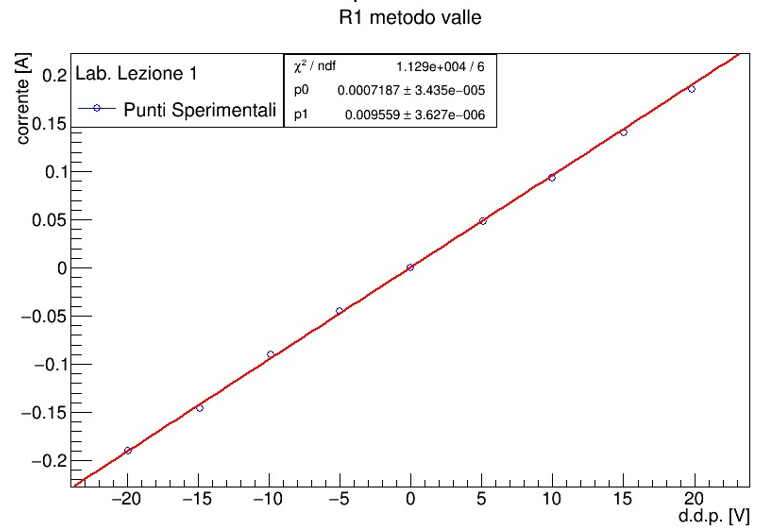
\includegraphics[width=\linewidth]{rel1-grafico_r1valle.png}
    \caption{Grafico di tensione e corrente relativi alla resistenza di valore nominale
di 100$\Omega$, ottenuto con il metodo a valle}
    \label{figura5}
\end{figure}
Per quanto riguarda il diodo, come è possibile osservare nel grafico, non è
possibile notare alcuna analogia con la legge di Ohm. Ciò accade perché la
corrente può scorrere solo in un verso prestabilito e, inoltre, la dipendenza tra
tensione ai capi e intensità di corrente non è lineare. E' utile sottolineare che
nel circuito è stato introdotta una resistenza di protezione in serie con il LED,
in modo da evitare danni al dispositivo circuitale.
\begin{figure}
    \centering
    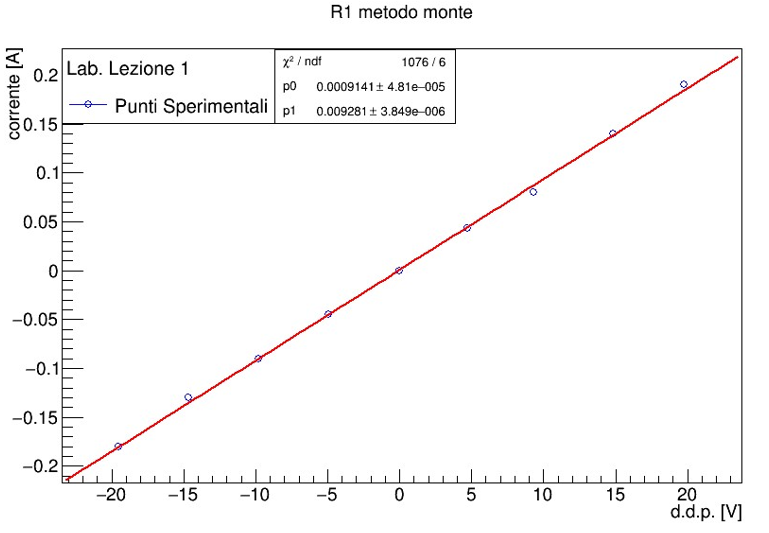
\includegraphics[width=\linewidth]{rel1-grafico_r1monte.png}
    \caption{Grafico di tensione e corrente relativi alla resistenza di valore nominale
di 100$\Omega$, ottenuto con il metodo a monte}
    \label{figura6}
\end{figure}
\begin{figure}
    \centering
    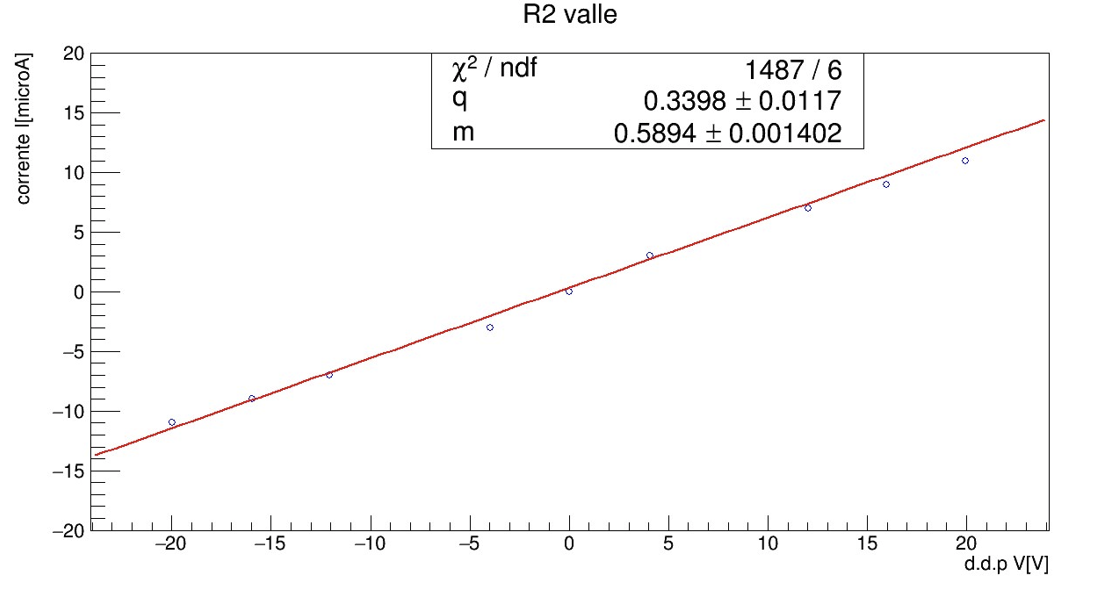
\includegraphics[width=\linewidth]{rel1-grafico_r2valle.png}
    \caption{Grafico di tensione e corrente relativi alla resistenza di valore nominale
di 2.2M$\Omega$, ottenuto con il metodo a valle}
    \label{figura7}
\end{figure}
\begin{figure}
    \centering
    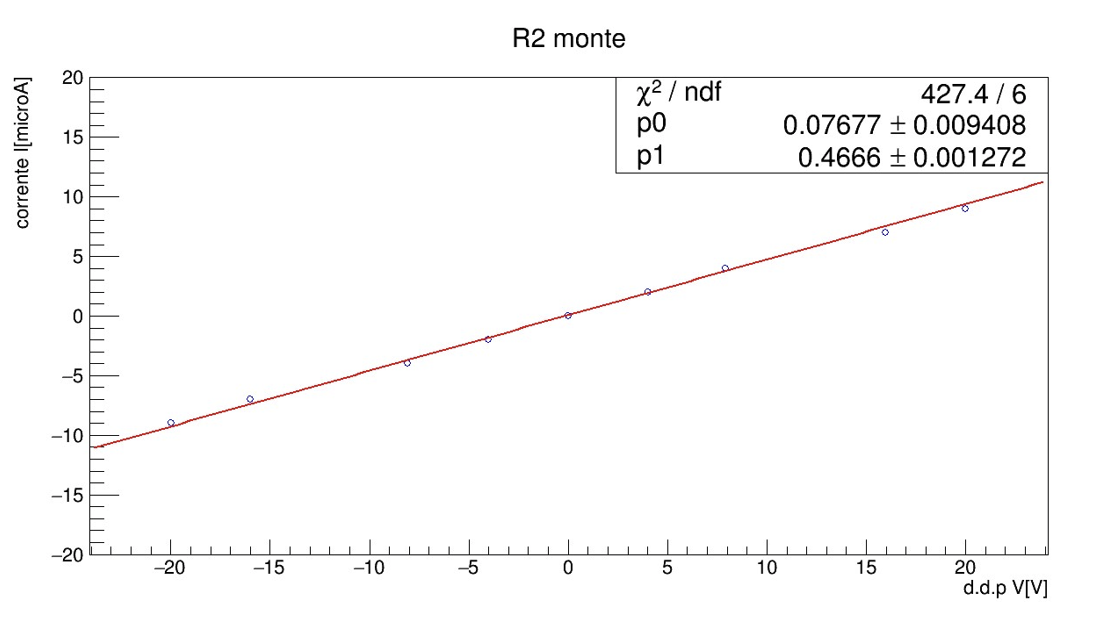
\includegraphics[width=\linewidth]{rel1-grafico_r2monte.png}
    \caption{Grafico di tensione e corrente relativi alla resistenza di valore nominale
di 2.2M$\Omega$, ottenuto con il metodo a monte}
    \label{figura8}
\end{figure}
\begin{figure}
    \centering
    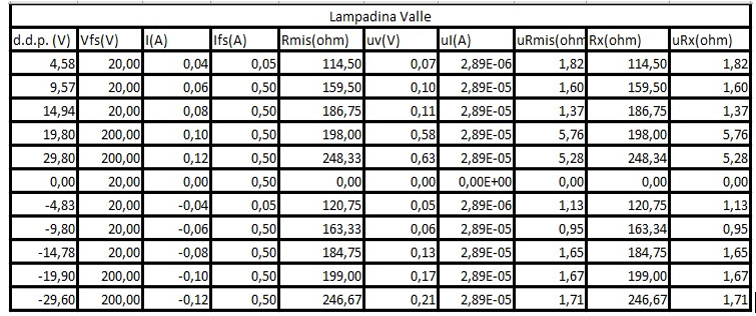
\includegraphics[width=\linewidth]{rel1-tabella_lampadina.png}
    \caption{Dati di tensione e corrente relativi alla lampadina ad incandescenza}
    \label{figura9}
\end{figure}
\begin{figure}
    \centering
    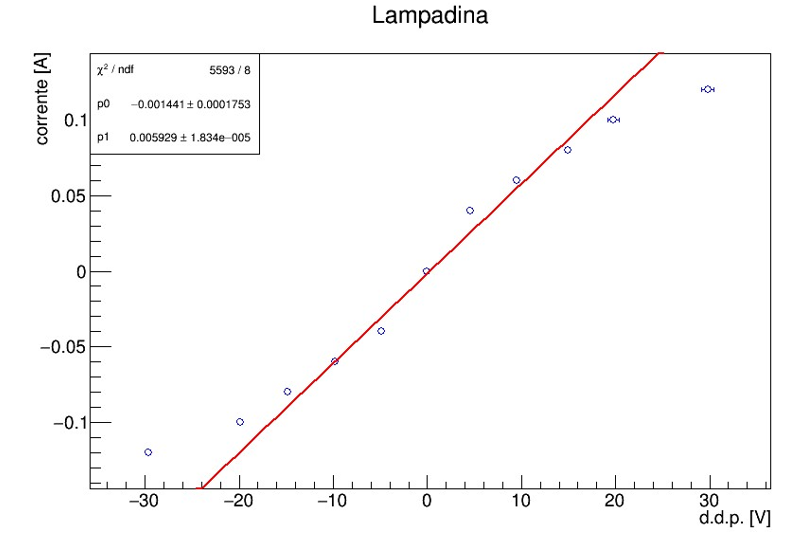
\includegraphics[width=\linewidth]{rel1-grafico_lampadina.png}
    \caption{Grafico di tensione e corrente relativi alla lampadina ad incandescenza}
    \label{figura10}
\end{figure}
\begin{figure}
    \centering
    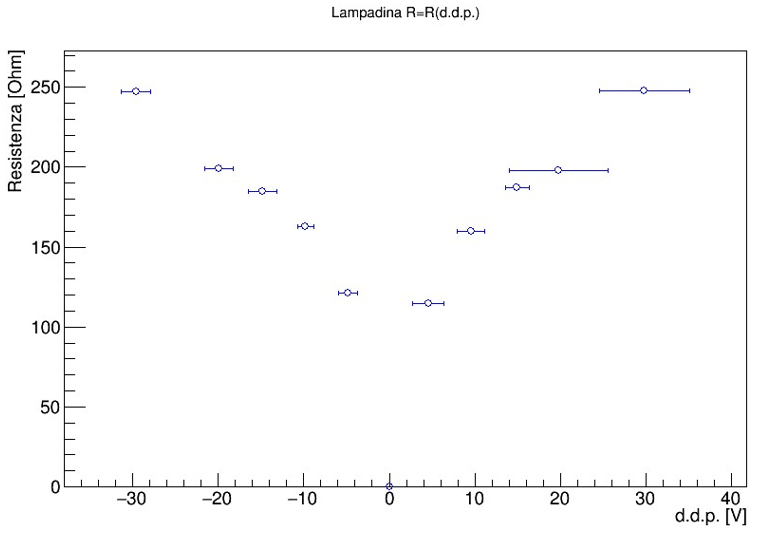
\includegraphics[width=\linewidth]{rel1-grafico_resistenza_lampadina.png}
    \caption{Andamento della resistenza in funzione della d.d.p. per la lampadina.}
    \label{figura11}
\end{figure}
\begin{figure}
    \centering
    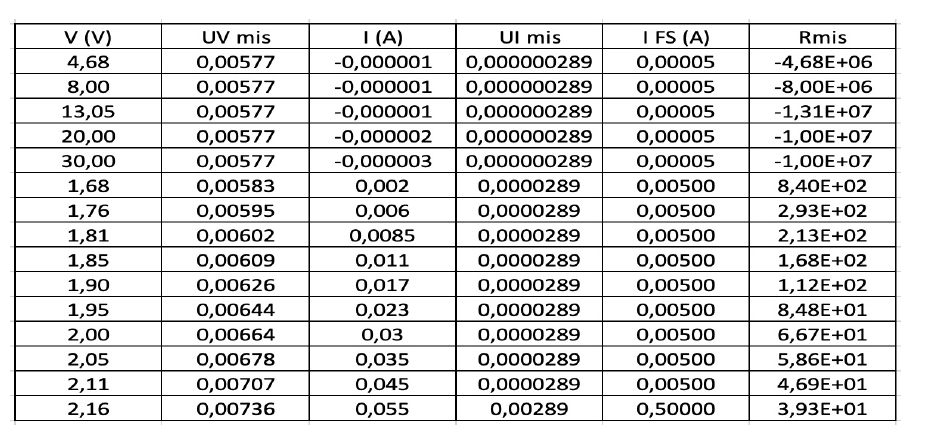
\includegraphics[width=\linewidth]{figura11.png}
    \caption{Dati di tensione e corrente relativi al diodo LED}
    \label{figura12}
\end{figure}
\begin{figure}
    \centering
    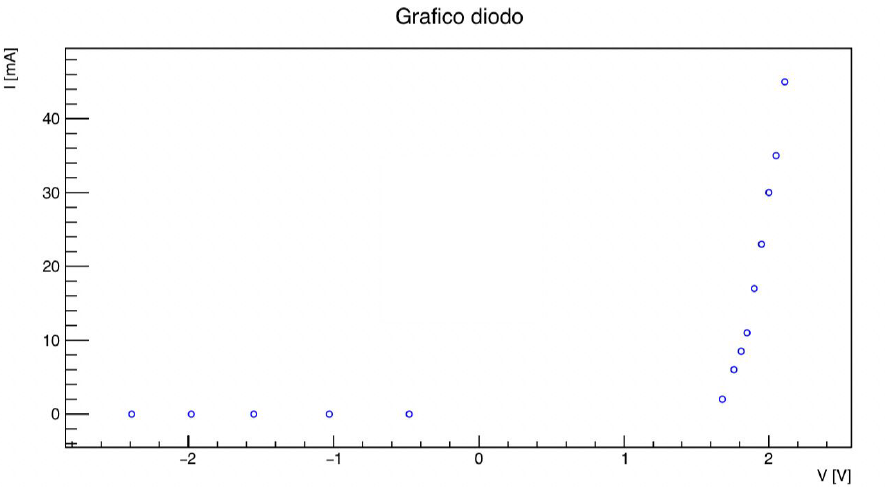
\includegraphics[width=\linewidth]{figura12.png}
    \caption{Grafico di tensione e corrente relativi al diodo LED}
    \label{figura13}
\end{figure}


\end{document}
